\subsection{Opgaver}

\begin{enumerate}
	\item Bestem $f'(1)$ for funktionen $f(x)=3x^3+\frac{1}{2}x^2-1$.

	\item Brug regnereglen $\frac{d}{dx} x^n=nx^{n-1}$ til at differentiere funktionerne
	\begin{align*}
	f(x)=x^3,&& f(x)=3+x,&& f(x)=\sqrt{x},&& f(x)=\frac{1}{x},&& f(x)=2x^6.
	\end{align*}
	
	\item Differentier funktionerne 
	\begin{align*}
	f(x)=3e^{2x}-\frac{1}{2}\ln x,&& f(x)=\frac{1}{2}\sin x,&& f(x)=\ln(\frac{x^2}{13})+3e^{-\frac{1}{12}x}
	\end{align*}
	
	\item Differentier funktionerne
	\begin{align*}
	f(x)=3x^7+2x^4-3x^2,&&f(x)=2x^5+3x^{\frac{3}{2}}-2x^{-2},&&f(x)=3\sqrt{x}+\frac{1}{x}.
	\end{align*}
	
		
	\item \label{it:diff12} Bestem for hver af de blå grafer i Figur~\ref{fig:diff12} hvilken af de røde grafer der beskriver den afledede.
	\begin{figure}
		\centering
		
		\begin{minipage}{0.3\linewidth}
			\begin{tikzpicture}[scale=0.5]
			\begin{axis}[xmin=-2,xmax=2,ymin=-2,ymax=2,axis x line=center,
			axis y line=center,ticks=none,xlabel={},ylabel={}]
			\addplot[thick,blue, samples = 600] {3/4*x^3+7/8*x^2-7/8*x-3/4};
			\end{axis}
			\end{tikzpicture}
		\end{minipage}
		\begin{minipage}{0.3\linewidth}
			\begin{tikzpicture}[scale=0.5]
			\begin{axis}[xmin=-2,xmax=2,ymin=-2,ymax=2,axis x line=center,
			axis y line=center,ticks=none,xlabel={},ylabel={}]
			\addplot[thick,blue, samples = 200] {-0.5*x-0.5};
			\end{axis}
			\end{tikzpicture}
		\end{minipage}
		\begin{minipage}{0.3\linewidth}
			\begin{tikzpicture}[scale=0.5]
			\begin{axis}[xmin=-2,xmax=2,ymin=-2,ymax=2,axis x line=center,
			axis y line=center,ticks=none, restrict y to domain=-2:2,xlabel={},ylabel={}]
				\addplot[thick,blue, samples = 600] {sqrt(x+2)-1};
			\end{axis}
			\end{tikzpicture}
		\end{minipage}
		\begin{minipage}{0.3\linewidth}
			\begin{tikzpicture}[scale=0.5]
			\begin{axis}[xmin=-2,xmax=2,ymin=-2,ymax=2,axis x line=center,
			axis y line=center,ticks=none,xlabel={},ylabel={}]
				\addplot[thick,red, samples = 600] {1/(2*sqrt(x+2))};
			\end{axis}
			\end{tikzpicture}
		\end{minipage}
		\begin{minipage}{0.3\linewidth}
			\begin{tikzpicture}[scale=0.5]
			\begin{axis}[xmin=-2,xmax=2,ymin=-2,ymax=2,axis x line=center,
			axis y line=center,ticks=none,xlabel={},ylabel={}]
			\addplot[domain=-2:2,thick,red, samples = 600] {9/4*x^2+7/4*x-7/8};
			\end{axis}
			\end{tikzpicture}
		\end{minipage}
		\begin{minipage}{0.3\linewidth}
			\begin{tikzpicture}[scale=0.5]
			\begin{axis}[xmin=-2,xmax=2,ymin=-2,ymax=2,axis x line=center,
			axis y line=center,ticks=none,xlabel={},ylabel={}]
			\addplot[thick,red, samples = 200] {-0.5};					
			\end{axis}
			\end{tikzpicture}
		\end{minipage}
		\caption{Opgave~\ref{it:diff12}}
		\label{fig:diff12}
	\end{figure}	
	
	\item Brug \href{https://www.geogebra.org/m/eTmzBFEq}{Geogebra} til bestemme 
	\begin{align*}
	\lim_{h\to 0^+} \frac{f(1+h)-f(1)}{h}
	\end{align*}
	for funktionen
	\begin{align*}
	f(x)=\begin{cases}
	\frac{x}{x+3},&\textup{hvis } x\leq 1\\
	\frac{x}{x+3}+2,&\textup{hvis } x> 1.
	\end{cases}
	\end{align*}
	Hvorfor er $f$ ikke differentiabel i $x=1$?
	
	\item Brug definitionen af differentialkvotienten til at finde den afledede af funktionerne
	\begin{align*}
	f(x)=k,&&f(x)=x,&&f(x)=kx.
	\end{align*}
	
	\item Bestem, for hver af de følgende funktioner, de punkter hvor tangenthældningen er $2$.
	\begin{align*}
	f(x)=\frac{x^3-2x}{x},&& f(x)=\frac{1}{3}x^3-2x^2+2x+7,&& 
	\end{align*}
	
	\item Differentier funktionerne 
	\begin{align*}
	f(x)=3\sqrt[3]{x},&& f(x)=(2x-1)x^2,&& f(x)=(5x+3)(2x^2-2)(x+7).
	\end{align*}
	
	\item Lad $f(x)=2x^2-3x+1$ og $g(x)=x^3-3x^2+3x$. Bestem $(f+g)'(x)$ og $(f-g)'(x)$.
	
	\item Brug \href{https://www.geogebra.org/m/eTmzBFEq}{Geogebra} til bestemme 
	\begin{align*}
	\lim_{h\to 0^+} \frac{f(h)-f(0)}{h},\quad \textup{og}\quad \lim_{h\to 0^-} \frac{f(h)-f(0)}{h}
	\end{align*}
	 for funktionen
	\begin{align*}
	f(x)=1-x^{2/5}.
	\end{align*}
	Hvorfor er $f$ ikke differentiabel i $x=0$?
	
	\item Differentier funktionerne
	
	\begin{align*}
		f(x)=\frac{\sqrt{x}+1}{x},&& f(x)=\frac{x^2\sqrt{x^3}}{x^{-1/4}},&& f(x)=2\cos(\frac{x}{2})\sin(\frac{x}{2}),&&f(x)=\ln\frac{1}{x^2}
	\end{align*}
	
	

	
	\item \label{it:diff11} Bestem for hver af de blå grafer i Figur~\ref{fig:diff11} hvilken af de røde grafer der beskriver den afledede.
		\begin{figure}
		\centering
		
		\begin{minipage}{0.3\linewidth}
			\begin{tikzpicture}[scale=0.5]
			\begin{axis}[xmin=-2,xmax=2,ymin=-2,ymax=2,axis x line=center,
				axis y line=center,ticks=none,xlabel={},ylabel={}]
				\addplot[domain=0:2,thick,blue, samples = 600] {(x^2)^(1/3)};
				\addplot[domain=-2:0,thick,blue,samples=600] {((-x)^2)^(1/3)};
				\end{axis}
			\end{tikzpicture}
		\end{minipage}
		\begin{minipage}{0.3\linewidth}
			\begin{tikzpicture}[scale=0.5]
			\begin{axis}[xmin=-2,xmax=2,ymin=-2,ymax=2,axis x line=center,
			axis y line=center,ticks=none,xlabel={},ylabel={}]
			\addplot[thick,blue, samples = 200] {x*sqrt(2-x)};
			\end{axis}
			\end{tikzpicture}
		\end{minipage}
			\begin{minipage}{0.3\linewidth}
		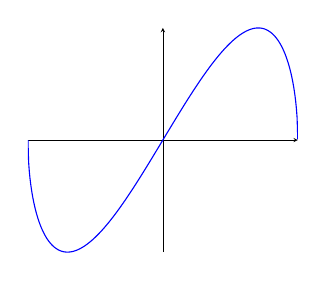
\begin{tikzpicture}[scale=0.5]
		\begin{axis}[xmin=-2,xmax=2,ymin=-2,ymax=2,axis x line=center,
		axis y line=center,ticks=none,xlabel={},ylabel={}]
		\addplot[domain=0:2,thick,blue, samples = 200] {x*sqrt(4-x^2)};
		\addplot[domain=-2:0,thick,blue, samples = 200] {x*sqrt(4-(x)^2)};
		\end{axis}
		\end{tikzpicture}
	\end{minipage}
		\begin{minipage}{0.3\linewidth}
	\begin{tikzpicture}[scale=0.5]
	\begin{axis}[xmin=-2,xmax=2,ymin=-2,ymax=2,axis x line=center,
	axis y line=center,ticks=none,xlabel={},ylabel={}]
	\addplot[thick,red, samples = 200] {sqrt(2-x)-x/(2*sqrt(2-x))};
	\end{axis}
	\end{tikzpicture}
\end{minipage}
\begin{minipage}{0.3\linewidth}
	\begin{tikzpicture}[scale=0.5]
	\begin{axis}[xmin=-2,xmax=2,ymin=-2,ymax=2,axis x line=center,
	axis y line=center,ticks=none,restrict y to domain=-2:2,restrict x to domain=-2:2,xlabel={},ylabel={}]
	\addplot[domain=0:2,thick,red, samples = 200] {sqrt(4-x^2)-x^2/sqrt(4-x^2)};
\addplot[domain=-2:0,thick,red, samples = 200] {sqrt(4-x^2)-x^2/sqrt(4-x^2)};
	\end{axis}
	\end{tikzpicture}
\end{minipage}
\begin{minipage}{0.3\linewidth}
	\begin{tikzpicture}[scale=0.5]
	\begin{axis}[xmin=-2,xmax=2,ymin=-2,ymax=2,axis x line=center,
	axis y line=center,ticks=none,restrict y to domain=-4:4,xlabel={},ylabel={}]
		\addplot[domain=0:2,thick,red, samples = 600] {2/3*(x)^(-1/3)};
		\addplot[domain=-2:0,thick,red, samples = 600] {-2/3*(-x)^(-1/3)};
	\end{axis}
	\end{tikzpicture}
	\end{minipage}
	\caption{Opgave~\ref{it:diff11}}
	\label{fig:diff11}
	\end{figure}	
	
	\item\label{it:diff13} Lad $f(x)=x-2\cos x$. 
	\begin{enumerate}
		\item Bestem alle punkter hvor $f'(x)=1$.
		\item Vis at alle punkter på formen $ (x,f(x)) $ hvor $x$ er som i del (a) ligger på en af de to linjer
		\begin{align*}
		y=x+2,\quad \textup{eller}\quad y=x-2.
		\end{align*}
	\end{enumerate}
	(Hint: Se Figur~\ref{fig:diff13}.)
	
	\begin{figure}
		\centering
		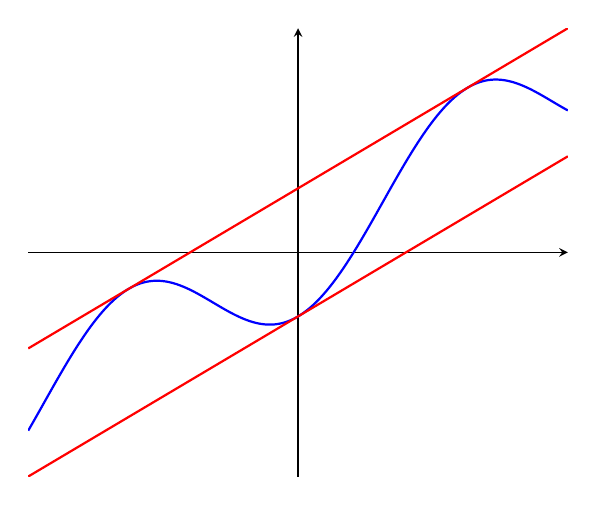
\begin{tikzpicture}
		\begin{axis}[axis x line=center,axis y line=center,ticks=none]
		\addplot[thick,blue, samples = 600] {x-2*cos(deg(x))};
		\addplot[thick,red, samples = 600] {x-2};
		\addplot[thick,red, samples = 600] {x+2};
		\end{axis}
		\end{tikzpicture}
		\caption{Opgave~\ref{it:diff13}}
		\label{fig:diff13}
	\end{figure}
	
	\item Brug definitionen af differentialkvotienten til at finde den afledede af funktionerne
	\begin{align*}
	f(x)=x^2,&&f(x)=\frac{1}{x},&&f(x)=\sin x&&, f(x)=\sqrt{x}
	\end{align*}
	(Hint: Brug sumformlerne, Opgave~\ref{it:lim1} og Opgave~\ref{it:lim3} til $\sin x$.)
	
	\item Differentier funktionerne
	\begin{align*}
	f(x)=-\ln(\frac{1}{x^3}),&& f(x)=\sqrt{e^{6x}}.
	\end{align*}
	
	\item \label{it:diff14} Lad $f\colon \R\to \R$ være givet ved
	\begin{align*}
	f(x)=\begin{cases}
	\frac{\sin x}{x},&\textup{hvis }x\neq 0\\
	1,&\textup{ellers}. 
	\end{cases}
	\end{align*}
	Brug definitionen af differentialkvotienten til at bestemme $f'(0)$. (Hint: Brug resultatet fra Opgave~\ref{it:lim4}.)
	
	\item\label{it:diff15} På Figur~\ref{fig:diff15} ses en cirkel med radius $r$ samt en tangent til cirklen som tangerer cirklen i punktet $P$. Lad $s$ betegne buelængden fra punktet $(1,0) $ til $ P $, lad $\theta$ betegne vinklen mellem vandret og tangenten og lad $\phi$ betegne vinklen mellem vandret og $P$.
	
	\begin{enumerate}
		\item Argumenter for at $\theta=\frac{\pi}{2}+\phi$.
		\item Brug formlen for længden af en cirkelbue, i.e. $ \phi r=s $, til at beskrive $ \theta $ som en funktion af $s$. 
		\item Vis at
		\begin{align*}
		\frac{d \theta}{d s}= \frac{1}{r}.
		\end{align*}
	\end{enumerate}
	
	\begin{figure}
		\centering
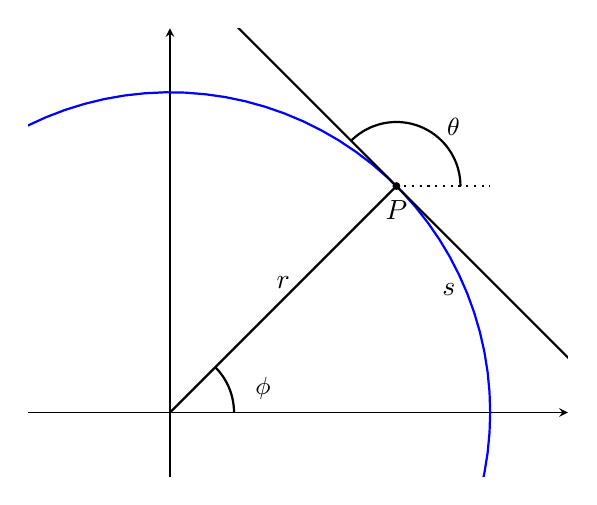
\begin{tikzpicture}
\begin{axis}[xmin=-0.2,xmax=1,ymin=-0.2,ymax=1.2,axis x line=center,
axis y line=center, axis equal,ticks =  none]
\pgfmathsetmacro\foo{sqrt(2)/2}
%\draw[fill=gray!40] (axis cs:0,0)--(axis cs:1,0)--(axis cs:\foo,\foo);		
%\draw[fill=gray!40] (axis cs:1,0)  arc[start angle=0, end angle=45,radius={transformdirectionx(1)}];

\addplot[blue,domain=0:2*pi,thick, samples=100] ({cos(deg(x))},{sin(deg(x))}) node[black,below,left,pos=0.0625] {$s$};
\addplot[domain=0:\foo,thick] {x} node[above,pos=0.5] {$r$};
\addplot[thick] {-x+2*\foo};
\addplot[domain=\foo:1,dotted,thick] {\foo};
\addplot[domain=0:pi/4,thick,samples=100] ({0.2*cos(deg(x))},{0.2*sin(deg(x))}) node[label={[label distance=2pt]0:\small$\phi$},pos=0.5] {};

\addplot[domain=0:3*pi/4,thick,samples=100] ({\foo+0.2*cos(deg(x))},{\foo+0.2*sin(deg(x))}) node[label={[label distance=2pt]0:\small$\theta$},pos=0.5] {};

\node[fill, circle, inner sep=1pt] at (axis cs:\foo,\foo) [label=below: $P$]{};
\end{axis}
\end{tikzpicture}
\caption{Opgave~\ref{it:diff15}}
\label{fig:diff15}
	\end{figure}
	\end{enumerate}